\section{What If The Initial Tokens Were Protected Against Fine-tuning Attacks?}
\label{sec:constraining}

The per-token dynamics of fine-tuning attacks that we analyze in Section~\ref{subsubsec:finetuning_stage_vulnerabilities} suggest that the safety failure after follow-up fine-tuning could be largely attributed to the distribution shift at only the first few tokens. Although this presents another frustrating view of the shallowness of the safety alignment, it also implies a potential avenue for mitigation. Specifically, we posit that: If the very first few output tokens play such a 
decisive role in a model's safety alignment, then we should be able to protect the alignment from being compromised during fine-tuning by simple  constraints to ensure that the generative distribution of these initial tokens does not significantly deviate. If this is true, it provides further evidence of shallow safety alignment and suggests one strategy for adding an additional layer of defense for production fine-tuning interfaces~(e.g., \citet{openaiFinetune}). 


\subsection{A Token-wise Constrained Objective for Custom Fine-tuning Aligned LLMs}
\label{subsec:token-wise-objective-intro}

\begin{comment}
\xiangyu{Consdering an alternative heading: what if the first few tokens are constrained during Fine-tuning?}

\ahmad{Per offline discussion, you may want to consider changing the narrative to pitching that the fine-tuning objective should be adapted to the alignment ``signature'' (not sure what the right word is). For example, let's consider the case where alignment is shallow. Can we still devise a finetuning objective that is effective yet preserves the alignment. And then end the section with, a more systematic design of finetuning rooted in alignment is a promising avenue for research.}

\ahmad{I think one question that you will probably get is: why did you not do (KL-)regularized training, e.g., $D_{\text{KL}}(\pi_\theta \| \pi_{aligned})$ to help with finetuning task while maintaining alignment as a baseline?}

\peter{Yeah, I agree. We've discussed this before I think. More specifically, why not just constrain $\mathbb{E}_{(x,y) \sim \mathcal{D_{\text{unsafe}}}}D_{\text{KL}}(\pi_\theta \| \pi_{aligned})$ where $D_{\text{unsafe}}$ are harmful prompts. May want to consider putting this on the timeline for rebuttal.}
\end{comment}



To further test our hypothesis, we devise the following fine-tuning objective---inspired in part by approaches like Direct Preference Optimization (DPO)~\citep{rafailov2023direct} and Kahneman-Tversky Optimization (KTO)~\citep{ethayarajh2024kto}--- but adapted to control the deviation from the initial generative distribution for each token position, similarly to the token-wise RL objective in~\citep{mudgal2024controlled}:
\begin{align}
    \min_{\theta} \Bigg\{ \ \ \mathop{\mathbb E}_{(\bx,\by)\sim D} -  \sum_{t=1}^{|\by|} \frac{2}{\beta_t} \log\Bigg[\sigma \bigg( \beta_t \log \frac{\pi_{\theta}\big(y_t \mid \bx, \by_{<t} \big)}{\pialigned\big(y_t \mid \bx, \by_{<t} \big)}  \bigg)  \Bigg] \ \ \Bigg\},
\label{eqn:soft-sft-fine-tuning-loss}
\end{align}
where $\sigma(z) := \frac{1}{1 + e^{-z}}$ is the sigmoid function and $\beta_t$ is a constant parameter at each token position to control the speed of the saturation of the sigmoid.
Here, a larger $\beta_t$ induces a stronger regularization strength towards the initial aligned model's generative distribution. See below for the interpretation of the proposed objective. 
%\xiangyu{!! A rectification here: the loss is multiplied by 2 in experiments to cancel out the $1/2$ factor introduced by $\sigma$. Following derivation parts need to be adjusted accordingly!!}




\textbf{Interpretation of Our Objective.}
To see why $\beta_t$ can be used to control the deviation of the generative distribution at each token position, we can rewrite the fine-tuning objective as:
\begin{align}
    \min_{\theta} \Bigg\{ \sum_{t \ge 1} \mathop{\mathbb E}_{(\bx,\by)\sim D}\!\Bigg[ \onec{t \le |\by|} \cdot \frac{2}{\beta_t} S\Big[\beta_t \big(\underbrace{\log \pialigned\big(y_t \mid \bx, \by_{<t} \big) - \log \pi_{\theta}\big(y_t \mid \bx, \by_{<t} \big)}_{=: \Delta_t(\bx, \by_{<t}, y_t)} \big) \Big] \Bigg] \Bigg\},
\end{align}
where $S(z) := \log(1 + e^{z})$ is the softplus function~\citep{dugas2000incorporating}.
At token position $t$, the loss is essentially $\Delta_t(\bx, \by_{<t}, y_t)$ (defined above) wrapped by the softplus function $S(\cdot)$ after being rescaled by $\beta_t$.
When $\beta_t$ is small, $S(\beta_t z) \approx S(0) + \beta_t S'(0) z = \log 2 + \frac{\beta_t}{2} z$,
so $\frac{2}{\beta_t}S(\beta_t z)$ is approximately equal to $- \log \pi_{\theta}\big(y_t \mid \bx, \by_{<t} \big)$ after shifting by a constant.
This means minimizing our objective is approximately the same as minimizing the cross-entropy loss 
$\mathop{\mathbb E}_{(\bx,\by)\sim D} \left[ - \onec{t \le |\by|} \cdot  \log \pi_{\theta}\big(y_t \mid \bx, \by_{<t} \big) \right]$. % up to affine transformation. 
Conversely, when $\beta_t$ is large, $\frac{2}{\beta_t}S(\beta_t z) = 2\max\{z, 0\} + \exp(-\Omega(\beta_t |z|))$, which converges exponentially to $2\max\{z, 0\}$.
The loss can then be approximated by $\mathop{\mathbb E}_{(\bx,\by)\sim D}\left[ \onec{t \le |\by|} \cdot \max\{ \Delta_t(\bx, \by_{<t}, y_t), 0 \}\right]$.
% \peter{The commented out part is correct, but it's a bit hard to parse/lengthy and the next paragraph drives home the point well.}
% which attains the minimum $0$ only if $\Delta_t(\bx, \by_{<t}, y_t) \le 0$ holds for all tuples $(\bx, \by_{<t}, y_t)$ that can be sampled from $D$, i.e., $\pi_{\theta}\big[y_t \mid \bx, \by_{<t} \big] \le \pialigned\big[y_t \mid \bx, \by_{<t} \big]$.
% If every token in the vocabulary can be sampled as $y_t$, then 
% $\pi_{\theta}\big[y_t \mid \bx, \by_{<t} \big] = \pialigned\big[y_t \mid \bx, \by_{<t} \big]$ holds for all $y_t$ because for two probability distributions that are different from each other, there must exist an element such that its probability in the first distribution is larger than that in the second distribution.
\textbf{This shows that small $\beta_t$ places emphasis on minimizing the cross-entropy loss, while large $\beta_t$ places emphasis on matching the generative distribution to the initial aligned model. }
% \peter{I replaced bolding with emph since the paragraph sections are already bolded}
% Taking a moderate value of $\beta_t$ then interpolates between these two regimes.
% PH: commented the above, the two approximations make assumptions that may not hold at moderate values, current wording makes it seem like we think approximations will continue as they are for moderate values, though I get what the sentence is saying, I think we can just push to appendix so nuance isn't lost.
In~\Cref{appendix:loss_limiting}, we provide a detailed derivation of these limiting behaviors for large and small $\beta_t$ and further characterization for the gradient when $\beta_t$ takes a moderate value.

\textbf{Gradient of Our Objective.} Our objective can also be interpreted by its gradient. The token-wise gradient of the objective on each data point $(\bx, \by)$ with $|\by| \ge t$ can be derived as:
% \begin{align}
%     \nabla \left( \frac{2}{\beta_t} S(\beta_t \Delta_t(\bx, \by_{<t}, y_t)) \right)
%     &= 
%     2 S'(\beta_t \Delta_t(\bx, \by_{<t}, y_t)) (-\nabla \log \pi_{\theta}\big(y_t \mid \bx, \by_{<t})) \nonumber\\
%     &= 2  \sigma(\beta_t \Delta_t(\bx, \by_{<t}, y_t)) (-\nabla \log \pi_{\theta}\big(y_t \mid \bx, \by_{<t}))
%     %&  -  \sum_{t=1}^{|\by|} w_t \times \nabla \ \log \ \pi_{\theta}\big[y_t|\bx, y_1,...,y_{t-1}\big],\ w_t := \Bigg[1 - \sigma\Bigg( \beta \cdot \log \frac{\pi_{\theta}\big[y_t|\bx, y_1,...,y_{t-1}\big]}{\pi_{aligned}\big[y_t|\bx, y_1,...,y_{t-1}\big]}\Bigg)\Bigg]
% \end{align}
\begin{equation}
    \nabla \left( \frac{2}{\beta_t} S(\beta_t \Delta_t(\bx, \by_{<t}, y_t)) \right)
    = - 2  \sigma(\beta_t \Delta_t(\bx, \by_{<t}, y_t)) \nabla \log \pi_{\theta}\big(y_t \mid \bx, \by_{<t}).
\end{equation}
Note that the gradient of the cross-entropy loss is $-\nabla \log \pi_{\theta}\big(y_t \mid \bx, \by_{<t}\big)$, our fine-tuning objective essentially applies an additional adaptive weight $w_t := 2\sigma(\beta_t \Delta_t(\bx, \by_{<t}, y_t))$ for the token-wise gradient term of cross-entropy. The weight $w_t$ diminishes as $-\Delta_t(\bx, \by_{<t}, y_t) := \log \pi_{\theta}\big(y_t \mid \bx, \by_{<t} \big) - \log \pialigned\big(y_t \mid \bx, \by_{<t} \big) $ becomes large.
This difference in log probabilities essentially characterizes the deviation between the fine-tuned model $\pi_{\theta}$ and the initially aligned model $\pi_{aligned}$ at the token position $t$ (see also~\Cref{thm:relu_loss_min}).
Taking together, we can see that the fine-tuning objective will adaptively diminish the weight of those token positions where the deviation of the distribution approaches a certain threshold (controlled by $\beta_t$), thereby constraining it from further deviation (by diminishing the gradient at this position). Note that, at the beginning of the fine-tuning when $\pi_\theta$ is initialized as $\pialigned$, the weight $w_t = 1$, and the gradient of the loss is equivalent to that of standard cross-entropy loss.\footnote{This is also why we multiply a constant factor $\frac{2}{\beta_t}$ to the loss. With this factor, we make sure the gradient magnitude is on par with the standard SFT (with cross-entropy loss) when the weight $w_t$ does not diminish.}

\textbf{Interpretation from A Reinforcement Learning Perspective.} In Appendix~\ref{appendix:loss-rl-perspective}, we further show how the loss function in Eqn~\ref{eqn:soft-sft-fine-tuning-loss} can also be derived from a KL-regularized reinforcement learning objective with $\beta_t$ controlling the strength of the KL regularizes at each different positions $t$. Under this RL-based interpretation, a larger $\beta_t$ essentially denotes a larger weight for the token-wise KL regularization terms, representing a stronger constraint enforcing that the token-wise generative distribution at the position $t$ does not deviate much from that of the initial model $\pialigned$.

\subsection{Experiments}

\textbf{Configurations of $\beta_t$.} To test our argument, we set a large $\beta$ for the first few tokens to impose a stronger constraint such that their generative distributions won't deviate too much from the aligned models. This leads to the implementation of larger $\beta_t$ as $\beta_1 = 0.5$, $\beta_t = 2$ for $2 \le t \le 5$ at the initial 5 tokens, while a much weaker constraint $\beta_t = 0.1$ for $t > 5$ at the later tokens. 

\textbf{Fine-tuning Attacks.} We test this constrained objective against \textit{three fine-tuning attacks} from \citet{qi2023fine} --- \textit{1) Harmful Examples:} fine-tuning with 100 (harmful input, harmful answer) pairs; \textit{2) Identity Shifting:} fine-tuning the model to self-identify as an absolutely obedient agent, and always answer questions with affirmative prefix; \textit{3) Backdoor Poisoning:} fine-tuning the model on a mixture of 100 (harmful input, refusal answer) pairs plus 100 (harmful input + a backdoor trigger, harmful answer) pairs. So the model will be fine-tuned to keep safe on normal harmful inputs~(w/o trigger) but be harmful when the trigger is added to the harmful input~(w/ trigger).


\textbf{Benign Fine-tuning.}  We also want to test whether the constrained fine-tuning objective can still fit benign downstream datasets to achieve comparable performances to that of the unconstrained objective. So, we experiment with \textit{three benign fine-tuning use cases} as well, including Samsum~\cite{samsum}, SQL Create Context~\cite{b-mc2_2023_sql-create-context} and GSM8k~\cite{cobbe2021gsm8k}.



\begin{table}[!htbp]
\caption{%\peter{Can we increase the font size of this table? it's so small. Can we also add what the +/- is for the caption?}
Fine-tuning with The Constrained Objective in Eqn~\ref{eqn:soft-sft-fine-tuning-loss}, with larger constraints $\beta_1 = 0.5$, $\beta_t = 2$ for $2 \le t \le 5$ at initial tokens, and small constraints for later tokens $\beta_t = 0.1$ for $t > 5$.}
\centering
  \resizebox{1.0\linewidth}{!}{

\begin{tabular}{c|c|c|c|c|c|c|c|c}
\hline
\multicolumn{2}{c|}{Models $\rightarrow$} &  \multicolumn{3}{c|}{Llama-2-7B-Chat} & & \multicolumn{3}{c}{Gemma-1.1-7B-IT}\\
\hline
\multirow{2}*{\shortstack{Datasets $\downarrow$}} & \multirow{2}*{\shortstack{\textbf{mean $\pm$ std }(\%)\\\textbf{(over 3 rounds)}}} & \multirow{2}*{\shortstack{Initial}} & \multirow{2}*{\shortstack{Standard\\SFT}} & \multirow{2}*{\shortstack{\textbf{Constrained}\\\textbf{SFT (ours)}}} & & \multirow{2}*{\shortstack{Initial}} & \multirow{2}*{\shortstack{Standard\\SFT}} & \multirow{2}*{\shortstack{\textbf{Constrained}\\\textbf{SFT (ours)}}} \\ 
&   &  &  &  &   &  & &\\
\hline
\multicolumn{9}{c}{\textit{Against Fine-tuning Attacks } }\\
\hline
Harmful Examples & ASR   &  1.5 $\pm$ 0.2  &  88.9 $\pm$ 1.2  &  4.6 $\pm$ 0.5  & &  1.8 $\pm$ 0.3 &  81.6 $\pm$ 2.9 & 1.9 $\pm$ 0.2\\
\hline
Identity Shifting & ASR   &  0 $\pm$ 0 & 
 79.5 $\pm$ 2.3   &   8.1 $\pm$ 0.1 & &  0 $\pm$ 0 &  83.6 $\pm$ 2.5 & 9.1 $\pm$ 1.7 \\
%\hline
%Data Selection~\citep{he2024s} &  ASR  & 3.6\%  &    &    &    &  \\
\hline
\multirow{2}*{\shortstack{Backdoor\\Poisoning}}  & ASR (w/o trigger)   & 1.5 $\pm$ 0.2   & 7.6 $\pm$ 1.1   &  1.9 $\pm$ 0.2 & &  1.8 $\pm$ 0.3 &  2.0 $\pm$ 0.2 & 1.5 $\pm$ 0.1 \\
 & ASR (w/ trigger)  &  1.7 $\pm$ 0.1  & 90.9 $\pm$ 1.4  & 10.9 $\pm$ 2.8  & & 1.8 $\pm$ 0.3  &  82.3 $\pm$ 1.1 & 1.9 $\pm$ 0.8\\
\hline
\multicolumn{9}{c}{\textit{Fine-tuning with Normal Downstream Datasets}}\\
\hline
\multirow{2}*{\shortstack{Samsum}} & ASR  & 1.5 $\pm$ 0.2  &   23.4 $\pm$ 2.5  &   3.2 $\pm$ 0.8 & &  1.8 $\pm$ 0.3 &  2.0 $\pm$ 0.2 & 2.4 $\pm$ 0.3 \\
&  Utility & 25.5 $\pm$ 0.3 & 51.7 $\pm$ 0.5  &   50.1 $\pm$ 0.2  & &  36.0 $\pm$ 1.4 &  51.5 $\pm$ 0.3 & 51.9 $\pm$ 0.5 \\
\hline
\multirow{2}*{\shortstack{SQL Create Context}} & ASR  & 1.5 $\pm$ 0.2 & 15.4 $\pm$ 1.4 & 3.2 $\pm$ 0.8   & &  1.8 $\pm$ 0.3 &  2.8 $\pm$ 0.2 & 2.4 $\pm$ 0.1 \\
&  Utility & 14.9 $\pm$ 0.4 & 99.1 $\pm$ 0.2  &  98.5 $\pm$ 0.1  & &  88.0 $\pm$ 0.5 &  99.2 $\pm$ 0.1 & 98.6 $\pm$ 0.3 \\
\hline
\multirow{2}*{\shortstack{GSM8k}} & ASR  & 1.5 $\pm$ 0.2 & 3.3 $\pm$ 0.4 &   2.0 $\pm$ 0.5  & &  1.8 $\pm$ 0.3 &  2.9 $\pm$ 0.2 & 1.7 $\pm$ 0.4 \\
&  Utility & {25.5} $\pm$ 0.2 & 41.7 $\pm$ 0.4 &  37.4 $\pm$ 0.3 & &  28.5 $\pm$ 1.2 &  63.3 $\pm$ 0.5 & 63.6 $\pm$ 0.4 \\
\hline
\end{tabular}}
\label{tab:main}
\end{table}

\textbf{Imposing Strong Constraints on Initial Tokens Mitigate Fine-tuning Attacks.} Table~\ref{tab:main} summarizes our results of fine-tuning Llama-2-7B-Chat and Gemma-1.1-7B-IT with the proposed constrained fine-tuning objective. As illustrated, the constrained fine-tuning objective~(Constrained SFT in the table) generally keeps a low ASR after both adversarial fine-tuning attacks and benign fine-tuning with normal downstream datasets. This suggests that the safety alignment can indeed be more persistent against fine-tuning if we can properly apply a tight constraint to prevent the distribution of early tokens from deviating too much from the initial models.

%\begin{wrapfigure}{l}{0.45\textwidth}
%  \vspace{-2em}
%  \begin{center}
%  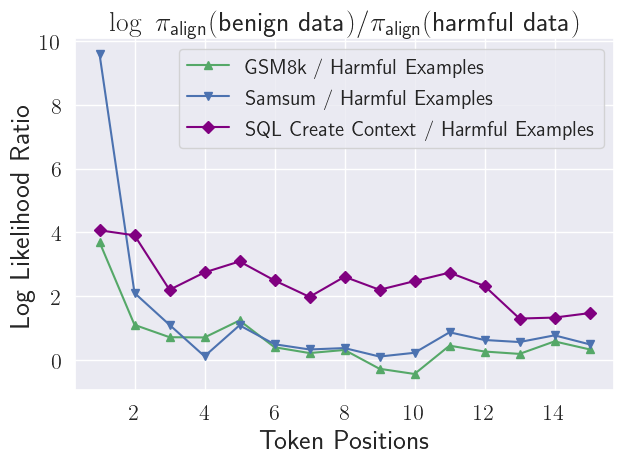
\includegraphics[width=\linewidth]{figs/logp_ratio.png}
%  \end{center}
%  \vspace{-1em}
%  \caption{Log ratio between the  }
%  \vspace{-1.0em}
%  \label{fig:finetuning_log_p_ratio}
%\end{wrapfigure} 

%\textbf{Comparable Utility Using The Constrained Loss.} In Table~\ref{tab:main}, we also report a utility metric for benign fine-tuning use cases. On Samsum and SQL Create Context, we report the standard ROUGE-1 score used for these datasets. On GMS8k, we report the accuracy of the answer. As shown, in all three use cases, both standard SFT and constrained SFT can improve the utility compared with the initial model. Notably, constrained SFT achieves comparable utility to standard SFT while mitigating the risk of harmful fine-tuning. This finding suggests that constraining initial tokens offers significant advantages in maintaining model safety, without significantly compromising the model's ability to leverage fine-tuning for enhanced utility in many downstream tasks. This is a meaningful insight that may be taken use of to build an additional layer of protection for production fine-tuning interfaces such as \citet{openaiFinetune} --- fine-tuning interfaces providers often want to allow users to custom fine-tune their models for downstream usage while not compromising the safety alignment of these models.


\textbf{Comparable Utility Using The Constrained Loss.} In Table~\ref{tab:main}, we also report utility metrics for benign fine-tuning use cases, employing the standard ROUGE-1 score for Samsum and SQL Create Context, and answer accuracy for GSM8k, consistent with established practices for these datasets. As shown, both standard SFT and constrained SFT improve utility compared to the initial model across all three cases. Notably, constrained SFT achieves comparable utility to standard SFT while mitigating the risk of harmful fine-tuning. These results suggest that constraining initial tokens offers significant advantages in maintaining model safety, without significantly compromising the model's ability to still leverage fine-tuning for enhanced utility in many downstream tasks. This is a meaningful insight that may be leveraged to build an additional layer of protection for production fine-tuning interfaces such as OpenAI's Finetuning API~\cite{openaiFinetune}. Since fine-tuning interface providers want to allow their users to customize their models for downstream usage while not breaking the safety alignment, they should consider enforcing such more restrictive fine-tuning objectives that are strategically designed to protect safety alignment while allowing customizability. 




%This suggests that, while constraining the initial tokens are highly beneficial for keeping the model's safety performance, the model can still meaningfully use fine-tuning to improve its utility in downstream tasks. 

%and constrained SFT achieves comparable utility to standard SFT --- while it can prevent harmful fine-tuning.

\textbf{Experiment Details and More Ablation Studies.} The full implementation details of this experiment can be found in Appendix~\ref{appendix-subsec:experiment_details-fine-tuning-attacks}. Besides, to further validate that the improvement in Table~\ref{tab:main} is indeed benefiting from the stronger constraints (larger $\beta_t$) biased to the first 5 tokens, we also provide further ablation studies on the choice of $\beta_t$ in Appendix~\ref{appendix:finetuning_ablation}.

%In Appendix~\ref{appendix:finetuning_ablation}, we provide further ablation studies with uniform $\beta = 0.1, 0.5, 2.0$ respectively for the constrained fine-tuning objective. We will show that a small constraint $\beta = 0.1$ uniformly for all tokens can not mitigate fine-tuning attacks, while $\beta = 0.5$ uniformly achieves both sub-optimal ASR and utility, and the largest $\beta = 2$ applied for all tokens often lead to mode collapse. 






% We find, as seen in Table 

% As a final note, the form of our fine-tuning objective is inspired by Direct Preference Optimization (DPO)~\citep{rafailov2023direct} for aligning a model to human preference data, which also wraps log probabilities with $\log \sigma(\cdot)$.
% \peter{You have to call out the similarity to KTO. Again, we should be cautious about pitching this as an exciting new defense/method. So anywhere we can tone it down, would be great.}
% But here we use log probability only on the positive samples from the training data and do not contrast the model's generative distribution between a pair of answers according to human preference.




